\documentclass{standalone}
\usepackage{tikz}
\usepackage{bm}
\renewcommand*\familydefault{\sfdefault}
\usepackage[italic]{mathastext}
\usepackage{isomath}

\def\wid{1.4cm}
\def\hei{5mm}

\begin{document}
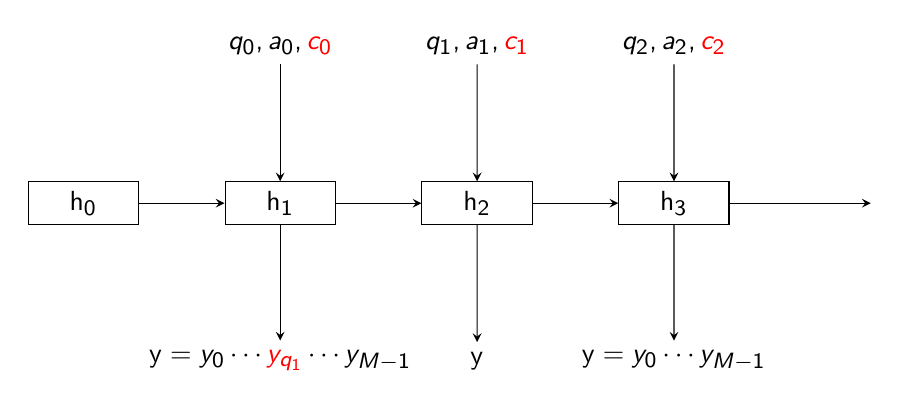
\begin{tikzpicture}[yscale=2,xscale=2.5,>=stealth]
\tikzset{->}
\node[draw,minimum width=\wid,minimum height=\hei,text centered] (h0) at (-1,-1) {$\bm{h_0}$};
\node (x0) at (0,0) {$q_0, a_0, \textcolor{red}{c_0}$};
\node (x1) at (1,0) {$q_1, a_1, \textcolor{red}{c_1}$};
\node (x2) at (2,0) {$q_2, a_2, \textcolor{red}{c_2}$};
\node[draw,minimum width=\wid,minimum height=\hei,text centered] (h1) at (0,-1) {$\bm{h_1}$};
% \node[draw,minimum height=\wid,text width=\hei,text centered,text depth=0pt,inner sep=1pt] (vq1) at (0.4,-1.5) {$v_{q_1}$};
\node[draw,minimum width=\wid,text centered] (h2) at (1,-1) {$\bm{h_2}$};
% \node[draw,minimum height=\wid,text width=\hei,text centered,text depth=0pt,inner sep=1pt] (vq2) at (1.4,-1.5) {$v_{q_2}$};
\node[draw,minimum width=\wid,text centered] (h3) at (2,-1) {$\bm{h_3}$};
% \node[draw,minimum height=\wid,text width=\hei,text centered,text depth=0pt,inner sep=1pt] (vq3) at (2.4,-1.5) {$v_{q_3}$};
\node (y1) at (0,-2) {$\bm{y} = y_0 \cdots \textcolor{red}{y_{q_1}} \cdots y_{M - 1}$};
\node (y2) at (1,-2) {$\bm{y}$};
\node (y3) at (2,-2) {$\bm{y} = y_0 \cdots y_{M - 1}$};
\draw (x0) to (h1);
\draw (x1) to (h2);
\draw (x2) to (h3);
\draw (h0) to (h1);
\draw (h1) to (h2);
\draw (h2) to (h3);
\draw (h3) to (3,-1);
\draw (h1) to (y1);
\draw (h2) to (y2);
\draw (h3) to (y3);
\end{tikzpicture}
\end{document}
